% The paper. AASTeX 7.0.1; compile with pdfLaTeX + BibTeX in this folder: latexmk -pdf main.tex
% The figures are the repository's own figures/ (see \graphicspath), as `belt-gradient run` writes them.
% After every edit run `python -I check_format.py` here and fix every FAIL (README.md lists the standards).
\documentclass[twocolumn]{aastex701}
\usepackage[T1]{fontenc}
\usepackage{array}
\usepackage{microtype}
\graphicspath{{../}} % figures/... resolve to the repository's figures/ folder
\hbadness=1000 % report loose lines (aastex701 sets 10000, hiding them)
% never hyphenate a cited surname (every plain-ASCII surname in refs.bib), a named statistic,
% or the word before a cross-reference number
\hyphenation{Aebersold Alexander Allard Audard Avdellidou Baraffe Bauer Berthier Binzel Bitsch Bolin Bottke Brasser Budde Burkhardt Cabrera Carruba Carry Carvano Casassus Cellino Chabrier Chambers Chang Chapman Chiang Christou Cieza Clark Clement Cloutis Connolly Crida Croix Cutri DeMeo Deienno Delbo Dermott Devillepoix Diniz Dones Dotto Dunham Edwards Efron Farinella Fornasier Golabek Gomes Gommers Gounelle Gradie Guillot Haisch Hands Hanley Harris Hartmann Hasselmann Hayashi Hiroi Homeier Hornoch Horvitz Hunter Izidoro Kehoe Kennedy Kenyon Kleine Kruijer Lauretta Lazzaro Lecar Levison Licandro Lichtenberg MacGibbon Mahlke Mainzer Mandell Masiero Mattei McCoy McKinney Milani Millman Minton Mojzsis Morbidelli Nagashima Nakai Nakamura Nimmo Noguchi Normand Nugent Observatoire Ockert Oliphant Onken Paolicchi Petit Pierens Pieters Podolak Popescu Pravec Propulsion Raymond Rivkin Robinson Rozehnal Rubincam Sasselov Sergeyev Slivan Sonnett Spoto Stevenson Sunshine Tanaka Tedesco Tholen Thompson Tobin Tsiganis Virtanen Walsh Warren Weidenschilling Winter Worsham Yokoyama Zolensky
  Kolmogorov Smirnov Bonferroni Hayabusa Itokawa Ryugu Bennu Figure Figures Table Tables Section Sections Equation Appendix AsteroidCatalog}
\raggedbottom
\makeatletter\def\raggedcolumn@sw#1#2{#1}\makeatother % balanced columns ragged, not stretched
\makeatletter % table notes read "Note.", not the class's "Note---" (aastex701.cls l. 11964)
\def\tablecomments#1{\vskip1pt{\small\vskip1sp\indent\vrule height 11pt depth 2pt
width 0pt\currtabletypesize{\sc Note.}\ {#1}\vskip1pt}}
\makeatother
\relpenalty=10000 \binoppenalty=10000 % never break inline math at = < > or a minus sign
\defcitealias{jpl2026}{Jet Propulsion Laboratory 2026}
\defcitealias{mp3c2026}{Observatoire de la C\^ote d'Azur 2026}
\shorttitle{Origin of the Main-Belt Compositional Gradient}
\shortauthors{Edwards}
\begin{document}
\title{Constraints on the Origin of the Asteroid Belt’s Compositional Gradient \texorpdfstring{\\}{}from Debiased Taxonomic Data}
\author[gname=Logan,sname=Edwards]{Logan M. Edwards}
\affiliation{Department of Aerospace, Physics, and Space Sciences, Florida Institute of Technology, Melbourne, FL 32901, USA}
\email[show]{ledwards2024@my.fit.edu}
\correspondingauthor{Logan M. Edwards}
\begin{abstract}
If asteroids formed at their present locations, the main belt should show a sharp change from dry S-types to hydrated C-types at the nebular snow line near 2.7~au. This prediction is tested with the 161,659 main-belt asteroids that have a published taxonomic classification, combined with the \citet{nesvornyetal2024} catalog of collisional families and proper elements. The catalog's other labels, 83\% of the main belt, are inferred from an albedo assigned by distance; they would reproduce the gradient by construction and are not used. Two corrections are essential. Collisional families are collapsed so that each disrupted parent body counts once, and the sample is limited by diameter rather than brightness, because a brightness-limited sample favors S-types. Uncorrected, the S/C crossover lies at 2.84~au, close to the snow line. After correction, two independent methods place it at $a_{50} = 2.41$–2.47~au, with a transition 1.4–1.5~au wide. The largest inner-belt bodies (over 100~km) are mostly S-type, but between about 10 and 100~km roughly half of inner-belt asteroids are carbonaceous. Measured albedos, independent of taxonomy, show the same gradient. \mbox{S-}~and C-types have indistinguishable proper eccentricities and inclinations in every zone except for one outer-belt difference that disappears once likely family-halo members are removed. A static condensation front cannot produce this pattern. A snow line that moved inward could broaden the transition, but cannot convert inner-disk material into the isotopically carbonaceous material sampled by C-types. The results therefore favor implantation of carbonaceous bodies from beyond Jupiter.
\end{abstract}
\keywords{\uat{Asteroid belt}{70}, \uat{Main belt asteroids}{2036}, \uat{Asteroid surfaces}{2209}, \uat{Hirayama families}{742}, \uat{Solar system formation}{1530}, \uat{Protoplanetary disks}{1300}}

\section{Introduction}\label{sec:1}
The Solar System can be read as a record of its own formation by asking of every observable whether it was set when the planets formed or altered afterward. The asteroid belt is particularly well suited to this question. Its bodies never assembled into a planet, most never melted, and their surfaces still record the composition of the solids in their region of the disk. The difficulty lies in establishing which region of the disk that was.

The best-known compositional feature of the belt is a gradient with heliocentric distance. \citet{gradie1982} found that bright, silicate-rich S-type asteroids dominate the inner belt while dark, carbon-rich C-types dominate the outer belt, and interpreted the pattern as evidence that the asteroids formed near their present locations. The standard explanation is the temperature structure of the solar nebula (\citealt{hayashi1981}). In a disk heated by the young Sun, the equilibrium temperature falls roughly as

\begin{equation}\label{eq:1}
T_{\mathrm{eq}} \simeq 278\ \mathrm{K}\left(\frac{a}{1\ \mathrm{au}}\right)^{-1/2},
\end{equation}
so water ice becomes stable ($T \approx 170$~K) beyond about 2.7~au (\citealt{hayashi1981}). In disk models that include accretion heating and realistic opacities, the snow line of a minimum-mass disk lies closer, near 1.6–1.8~au, and reaches 2.7~au only for higher opacity, accretion rate or disk mass (\citealt{lecar2006}). Solids that formed inside this snow line should be dry and thermally processed, and those that formed outside it should be ice-rich. If the asteroids still reside where they formed, the belt should show a transition from S to C near 2.7~au.

Several lines of evidence suggest otherwise. The belt today contains only about $5 \times 10^{-4}\,M_{\oplus}$, orders of magnitude less than a smooth extrapolation of the disk’s solid surface density would predict (\citealt{weidenschilling1977}), so most of its original material has been removed (\citealt{morbidelli2015}). Later surveys mapped the taxonomic distribution in much more detail (\citealt{mothediniz2003}; \citealt{demeo2013}) and found C-types in the inner belt and S-types in the outer belt (\citealt{demeo2014}; reviewed by \citealt{demeo2015}). Meteorites add a further constraint: their nucleosynthetic isotope anomalies divide them into non-carbonaceous (NC) and carbonaceous (CC) groups that remained separate for several million years, most plausibly because a growing Jupiter kept them apart (\citealt{warren2011}; \citealt{kruijer2017}; \citealt{kleine2020}). A long-lived pressure maximum in the gas disk near Jupiter’s orbit (\citealt{brasser2020}), or dust piling up at the snow line (\citealt{lichtenberg2021}), could also have kept the reservoirs apart, but in each of these scenarios the CC material formed farther from the Sun than the NC material. If the CC reservoir lay beyond Jupiter, the carbonaceous asteroids now in the belt most likely arrived from outside it.

Several dynamical models make this idea concrete. In the Grand Tack scenario, Jupiter migrates inward to about 1.5~au and then outward again, emptying the belt and then refilling it with S-types from the inner disk and C-types from beyond the giant planets (\citealt{walsh2011}). In the “empty belt” model, the belt never held much mass; it was filled by S-type planetesimals scattered outward from the terrestrial region and by C-types scattered inward during the rapid gas accretion of Jupiter and Saturn (\citealt{raymond2017a,raymond2017b}). Later, during the giant-planet instability (\citealt{tsiganis2005}), primitive \mbox{D-}~and P-type bodies from the trans-Neptunian region may have been captured into the outer belt (\citealt{levison2009}; \citealt{vokrouhlicky2016}). Other models deplete and excite the belt without a migrating Jupiter, through an early giant-planet instability (\citealt{clement2019}) or chaotic early orbits of Jupiter and Saturn (\citealt{izidoro2016}).

This paper asks whether the present-day gradient is primordial or the product of mixing. Plotting catalog labels against distance is not sufficient to answer this question, for three reasons that shape the method. Most labels in large catalogs are inferred rather than observed, and some are inferred in a way that assumes the answer. Collisional families inflate the counts with fragments of a few parent bodies. Finally, dark bodies are under-represented at any given brightness. Section~\ref{sec:2} sets out what each scenario predicts, Section~\ref{sec:3} describes the data and the corrections, Section~\ref{sec:4} presents the results, and Section~\ref{sec:5} discusses which scenarios they support or exclude.

\section{Background: \texorpdfstring{\\*}{}What Each Scenario Predicts}\label{sec:2}
\subsection{Taxonomy as a proxy for formation location}\label{sec:2.1}
Asteroid taxonomy classifies bodies by the shape of their visible and near-infrared reflectance spectra (\citealt{bus2002}; \citealt{demeo2009}). Two links make taxonomy useful for formation questions. Dust returned by Hayabusa from the S-type asteroid Itokawa matches ordinary chondrites (\citealt{nakamura2011}), which are NC meteorites. Samples returned by Hayabusa2 from the C-type asteroid Ryugu match CI chondrites (\citealt{yokoyama2023}), which are CC meteorites (\citealt{kleine2020}). To first order, therefore, S-types sample the NC reservoir and C-types sample the CC reservoir. The correspondence is imperfect: \mbox{K-}~and L-types are anhydrous but have been associated with CV and CO chondrites (\citealt{sunshine2008}; \citealt{clark2009}), and the X complex mixes metallic, enstatite-like and primitive bodies that cannot be distinguished without albedo (\citealt{demeo2013}).

\subsection{A moving snow line}\label{sec:2.2}
Equation~(\ref{eq:1}) describes a disk around a star of fixed luminosity, a condition that no protoplanetary disk meets. Gas disks last a few Myr (\citealt{haisch2001}), while a solar-mass star takes tens of Myr to contract onto the main sequence (\citealt{baraffe2015}), so throughout the disk’s gas-rich lifetime the star is more luminous than on the main sequence, and its luminosity declines. Together with declining accretion heating, this moves the snow line inward as the disk evolves (\citealt{kennedy2008}). Scaling Equation~(\ref{eq:1}) with the luminosity of the $1\,M_{\odot}$ track of \citet{baraffe2015}, the snow line moves from about 3.7~au at 1~Myr to about 2.1~au at 5~Myr, across the full width of the present belt (Figure~\ref{fig:1}): it first lies inside the belt’s outer edge (3.3~au) at 1.4~Myr and inside its inner edge (2.1~au) at 5.3~Myr. Superimposed on that drift are accretion outbursts of the FU Orionis type, in which the accretion rate rises from about $10^{-7}$ to a few $10^{-4}\,M_{\odot}$~yr$^{-1}$ and remains elevated for decades or longer (\citealt{hartmann1996}; \citealt{audard2014}). The disk responds within an outburst: in V883 Ori, a $1.3\,M_{\odot}$ protostar in outburst at about $400\,L_{\odot}$, the water snow line has been imaged at about 42~au (\citealt{cieza2016}).

\begin{figure}[htb!]
\centering
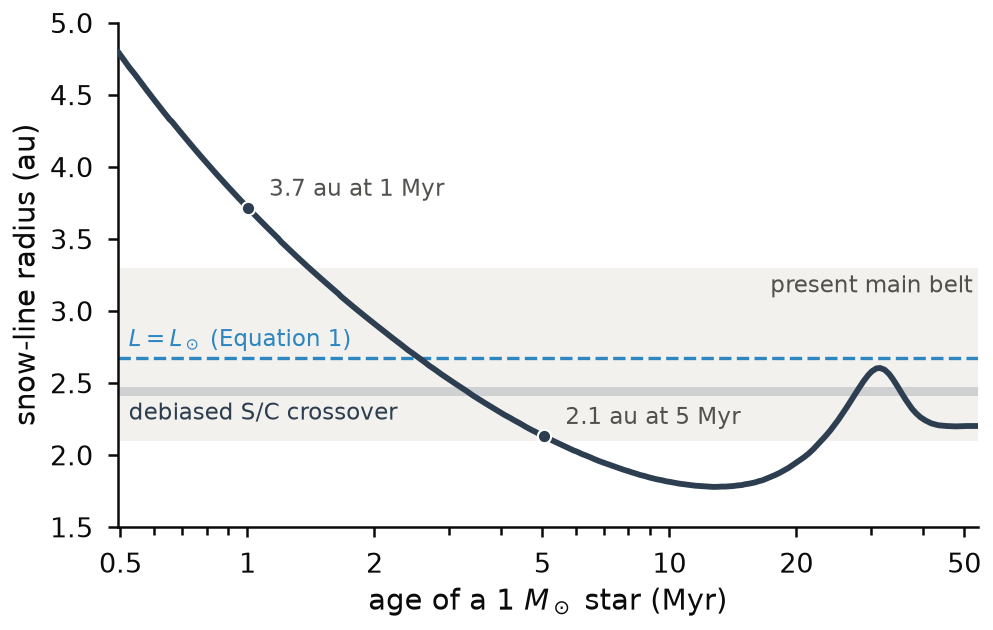
\includegraphics[width=\columnwidth]{figures/fig10_snow_line_track.png}
\caption{Snow-line radius from Equation~(\ref{eq:1}) scaled with the luminosity of a $1\,M_{\odot}$ pre-main-sequence star (\citealt{baraffe2015}), as a function of age. The light band is the present main belt, the darker band the debiased S/C crossover (Section~\ref{sec:4.4}), and the dashed line the snow line of Equation~(\ref{eq:1}) at the present solar luminosity.}\label{fig:1}
\end{figure}
Two consequences follow for the asteroid belt. First, the ice line sweeps through a band several au wide, and in that band a body’s water content can depend on \textit{when} it formed as much as on where. Whether ice actually reaches the inner part of that band depends on transport: as the snow line moves inward, water cannot condense directly from the local gas, and ice appears only where icy particles drift in from farther out, a flux that a growing Jupiter can interrupt (\citealt{morbidelli2016}). Second, a moving snow line changes only which volatiles condense. It cannot change the isotopic composition of the dust, which was set by which nucleosynthetic reservoir the material came from (\citealt{kleine2020}). In models where the migrating snow line helps create the two reservoirs, it does so by trapping inward-drifting dust, where it forms planetesimals, rather than by altering the isotopes of that dust (\citealt{lichtenberg2021}). This distinction becomes decisive in Section~\ref{sec:5.1}.

\subsection{Five scenarios}\label{sec:2.3}
Table~\ref{tab:1} summarizes the predictions this paper can test. The scenarios are not mutually exclusive; the capture proposed by \citet{levison2009} could have occurred in addition to either implantation model.

\begin{deluxetable*}{>{\raggedright\arraybackslash}p{1.5in}>{\raggedright\arraybackslash}p{2.0in}>{\raggedright\arraybackslash}p{3.15in}}
\tabletypesize{\footnotesize}
\tablewidth{0pt}
\tablecaption{Formation scenarios and their observable predictions.\label{tab:1}}
\tablehead{\colhead{Scenario} & \colhead{Reference} & \colhead{Prediction for the present belt}}
\startdata
Static condensation front & Equation~(\ref{eq:1}) & Narrow S$\rightarrow$C transition near 2.7~au; almost no C-types in the inner belt; composition unrelated to orbital excitation. \\
Moving snow line, in situ & Section~\ref{sec:2.2} & Broader transition; hydrated bodies in the inner belt possible, but made of inner-disk (NC) material. \\
Grand Tack & \citet{walsh2011,walsh2012} & Broad overlap: S concentrated inward, C outward, both dynamically excited during implantation. \\
Empty belt, implanted & \citet{raymond2017a,raymond2017b} & Broad overlap from both directions; C-types share a source with Earth’s water; belt stirred as a whole. \\
Late contamination & \citet{levison2009}; \citet{vokrouhlicky2016} & \mbox{D-}~and P-types concentrated in the outer belt, Hildas and Trojans.
\enddata
\end{deluxetable*}
The static front makes the sharpest prediction, and the asteroid data alone can test it: the transition should be much narrower than the 1.2~au span of the belt. The moving snow line is harder to test with asteroid data alone, because it predicts a broad transition too. What distinguishes it from the implantation models is the \textit{material} in the inner belt’s C-types, which must be assessed from meteorites.

\section{Data and Methods}\label{sec:3}
All analysis code is in a public Python repository, asteroid-belt-gradient (\citealt{edwards2026a}; release v2.6.3), built on NumPy (\citealt{harris2020}), SciPy (\citealt{virtanen2020}), pandas (\citealt{mckinney2010}) and Matplotlib (\citealt{hunter2007}). Two commands download the inputs and regenerate every figure and table in this paper, along with every number in the text that is derived from the data.

\subsection{The asteroid catalog and which labels to trust}\label{sec:3.1}
The starting point is a merged catalog of 1,568,882 asteroids, AsteroidCatalog (\citealt{edwards2026b}), built from NASA JPL’s Small-Body Database (\citetalias{jpl2026}), the SsODNet ssoBFT table (\citealt{berthier2023}), NEOWISE diameters and albedos (\citealt{mainzer2011a,mainzer2019}; \citealt{masiero2011,masiero2012,masiero2014,masiero2017}; \citealt{nugent2015,nugent2016}), and the Minor Planet Physical Properties Catalogue (MP3C; \citetalias{mp3c2026}), in its release of 2026 September 29 (tag \mbox{data-2026-09-29c}). The sample is restricted to the main belt: $2.1 < a < 3.3$~au with perihelion $q > 1.3$~au, which removes Mars-crossers. This leaves 1,443,761 bodies. The belt is divided at the 3:1, 5:2 and 7:3 mean-motion resonances with Jupiter into four zones: inner (2.1–2.5~au), middle (2.5–2.82~au), “pristine” (2.82–2.96~au; \citealt{brozetal2013}) and outer (2.96–3.3~au).

The catalog assigns a spectral type to almost every body, but by three different routes, and only one is usable here:

\begin{enumerate}
\item \textbf{Published taxonomy} (161,659 main-belt bodies): a classification compiled by SsODNet from photometric and spectroscopic surveys, mainly multi-filter colors from SkyMapper (\citealt{sergeyev2022}) and the Sloan Digital Sky Survey (SDSS; \citealt{carvano2010}; \citealt{demeo2013}; \citealt{sergeyev2021}), some near-infrared colors (\citealt{popescu2018}), and spectra for the brightest bodies (e.g., \citealt{bus2002}; \citealt{mahlke2022}). This is the primary sample.
\item \textbf{Measured albedo} (80,359 bodies): the geometric albedo $p_{\mathrm{V}}$ is thresholded ($p_{\mathrm{V}} < 0.10 \rightarrow$ C, otherwise S). Its labels are not used; measured albedos serve only as an independent check (Section~\ref{sec:4.6}).
\item \textbf{Assumed albedo} (1,201,743 bodies, 83\% of the belt): for bodies with no measured size, the catalog assumes an albedo from a lookup table indexed by semimajor axis (\citealt{edwards2026b}; 0.190 inside 2.5~au; 0.086, 0.066 and 0.057 beyond it) and then applies the same threshold.
\end{enumerate}
The third route is circular for this question. It assigns S inside 2.5~au and C outside by construction, so any analysis that uses it recovers the assumption. Figure~\ref{fig:2} shows the step function it produces. This route is therefore excluded entirely. The pitfall deserves emphasis because a catalog that appears complete can conceal it: the fraction of labels that are observed rather than inferred must be checked before a catalog is used to test a hypothesis about composition.

\begin{figure}[htb!]
\centering
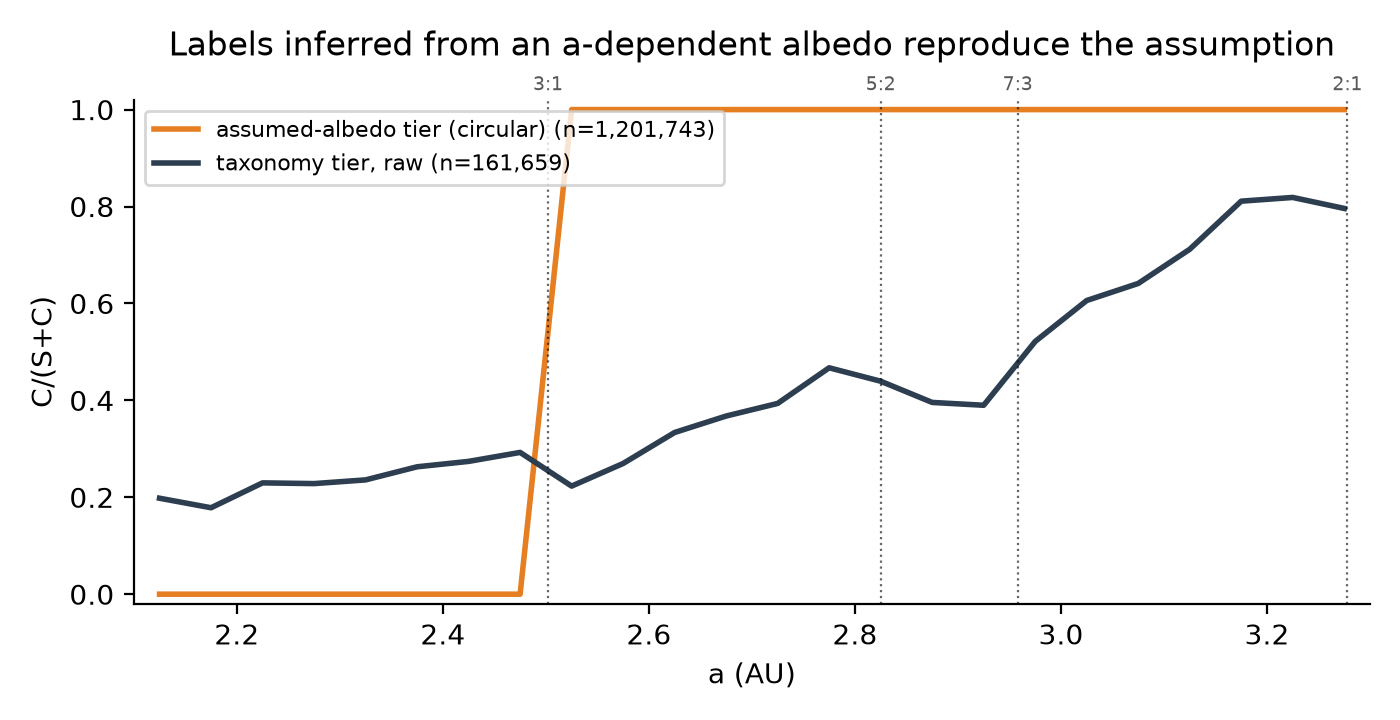
\includegraphics[width=\columnwidth]{figures/fig5_circularity.png}
\caption{C-fraction versus semimajor axis for labels inferred from an albedo that the catalog assigns by distance (orange), compared with published taxonomy (dark). The assumed-albedo labels return a step at 2.5~au because that is where the lookup table changes value. They are excluded from all analysis.}\label{fig:2}
\end{figure}
\subsection{Compositional groups}\label{sec:3.2}
Classes are grouped by their first letter: \textit{S-like} (S, Q, A, V, R, O), \textit{C-like} (C, B, F), \textit{D/P} (D, P, T, Z), \textit{K/L} (K, L), and \textit{X} (X, M, E). Two versions of the carbonaceous fraction are reported. The \textit{narrow} fraction is C/(S+C). The \textit{broad} fraction treats every group with a carbonaceous-chondrite affinity as carbonaceous (\citealt{hiroi2001}; \citealt{sunshine2008}; \citealt{clark2009}): (C+D/P+K/L)/(S+C+D/P+K/L). Without an albedo an X-type cannot be placed in the E, M or P class (Section~\ref{sec:2.1}), so X-types are excluded from both; Section~\ref{sec:4.6} tests the effect of splitting those that have a measured albedo. F is one of the minor classes of \citet{tholen1984}; Z is the class of extremely red main-belt objects introduced by \citet{mahlke2022}.

\subsection{Collisional families}\label{sec:3.3}
A collisional family is the debris of one parent body. The Vesta family alone contributes over 15,000 catalogued members. Counting fragments measures which bodies were disrupted rather than where each class formed, so families must be removed or collapsed.

Family membership comes from the hierarchical-clustering (HCM) catalog of \citet{nesvorny2015} and its 2024 update (\citealt{nesvornyetal2024}), distributed through the Small Bodies Node of NASA’s Planetary Data System (PDS) (\citealt{nesvorny2024}). The combined list has 272 families: 119 from 2015, plus 153 added in 2024, of which 136 are new discoveries. Proper elements are orbital elements with the periodic oscillations caused by the planets removed, so they are nearly invariant over time and the fragments of one parent remain clustered in them (\citealt{knezevic2003}; \citealt{nesvornyetal2024}). Families are identified as clusters in proper-element space ($a_{\mathrm{P}}$, $e_{\mathrm{P}}$, $\sin i_{\mathrm{P}}$) using the distance metric of \citet{zappala1990},

\begin{equation}\label{eq:2}
d = n a_{\mathrm{P}} \sqrt{\frac{5}{4}\left(\frac{\delta a_{\mathrm{P}}}{a_{\mathrm{P}}}\right)^{2} + 2(\delta e_{\mathrm{P}})^{2} + 2(\delta \sin i_{\mathrm{P}})^{2}},
\end{equation}
where $n a_{\mathrm{P}}$ is the orbital velocity, so $d$ is in m~s$^{-1}$. A body listed in two families (for example the young Karin cluster inside Koronis; \citealt{nesvorny2002}) is assigned to the larger family. Two pairs of lists in the archive are identical (the file for Vibilia repeats the members of Leonidas, and the 2024 families of 1998~HD$_{130}$ and 2001~PG$_{20}$ are the same bodies), so each pair counts as one family. In total, 153,271 main-belt bodies (10.6\%) are family members, but among bodies with a published taxonomy the fraction is 32.2\%, because family members are over-represented among well-observed asteroids.

Each family is then \textit{collapsed} to a single body. Its class is the most common group among its classified members other than X-types, provided at least three are classified and no two groups tie; otherwise the class of its largest member is used. Its diameter is the volume-equivalent $D_{\mathrm{eq}} = (\sum D_i^{3})^{1/3}$, and its position is that of its largest member. Collapsing, rather than deleting, keeps large parents such as Vesta and Hygiea in the sample once each. Of 240 families with main-belt members, 193 can be classified this way.

\subsection{Completeness and debiasing}\label{sec:3.4}
Taxonomic surveys are limited by brightness: spectroscopic targets were chosen by their visible brightness (\citealt{mainzer2011b}), and color surveys are complete only to a limiting magnitude (\citealt{sergeyev2022}). At a fixed absolute magnitude $H$, a dark C-type is larger than a bright S-type. Following \citet{pravec2007},

\begin{equation}\label{eq:3}
D = \frac{1329\ \mathrm{km}}{\sqrt{p_{\mathrm{V}}}} \times 10^{-H/5}.
\end{equation}
A sample limited in $H$ therefore over-represents S-types among small bodies, a bias also addressed by \citet{demeo2013}. The fraction of main-belt bodies with a published taxonomy is measured in bins of $H$ and zone (Appendix~\ref{app:completeness}, Figure~\ref{fig:A1}). It is at least 95\% in every zone for $H < 10.5$ and falls to about 60–75\% by $H \approx 14$. This bias is corrected in two independent ways.

\textbf{Size-complete sample. }Setting $H = 10.5$ and a very dark albedo $p_{\mathrm{V}} = 0.04$ in Equation~(\ref{eq:3}) gives $D_{\mathrm{c}} = 52.8$~km. Every body larger than $D_{\mathrm{c}}$ is brighter than $H = 10.5$ unless its albedo is below 0.04, so the sample of bodies with $D \geq D_{\mathrm{c}}$ is effectively complete. It is also small: 492 bodies after family collapse.

\textbf{Inverse-probability weighting (IPW). }Each classified body is weighted by $1/c(H, \mathrm{zone})$, the inverse of the completeness in its bin (\citealt{horvitz1952}), and the sample is limited to $D \geq 10$~km. Bins fainter than $H = 15$ or less than 30\% classified are not weighted, which removes a single body. The size limit is essential: weighting corrects for missing labels at a given brightness, but not for the S-bias of a sample defined by brightness. (Weighting a sample limited to $H < 15$ instead gives an inner-belt C-fraction of only 0.17.) At 10~km even a $p_{\mathrm{V}} = 0.04$ body has $H \approx 14.1$, where completeness is still substantial, so every body in the size range has a substantial probability of being classified. The method assumes that, at a fixed $H$ and zone, whether a body has been classified does not depend on its class.

Four samples are reported: \textit{raw} (all classified bodies, families included); \textit{collapsed, IPW,} $D \geq 10$~km; \textit{collapsed,} $D \geq 53$~km; and \textit{background only,} $D \geq 53$~km, in which family members are removed rather than collapsed. Uncertainties are 16–84\% intervals from a Poisson bootstrap (\citealt{efron1979}; \citealt{hanley2006}). Figure~\ref{fig:3} traces each sample back to the catalog.

\begin{figure}[htb!]
\centering
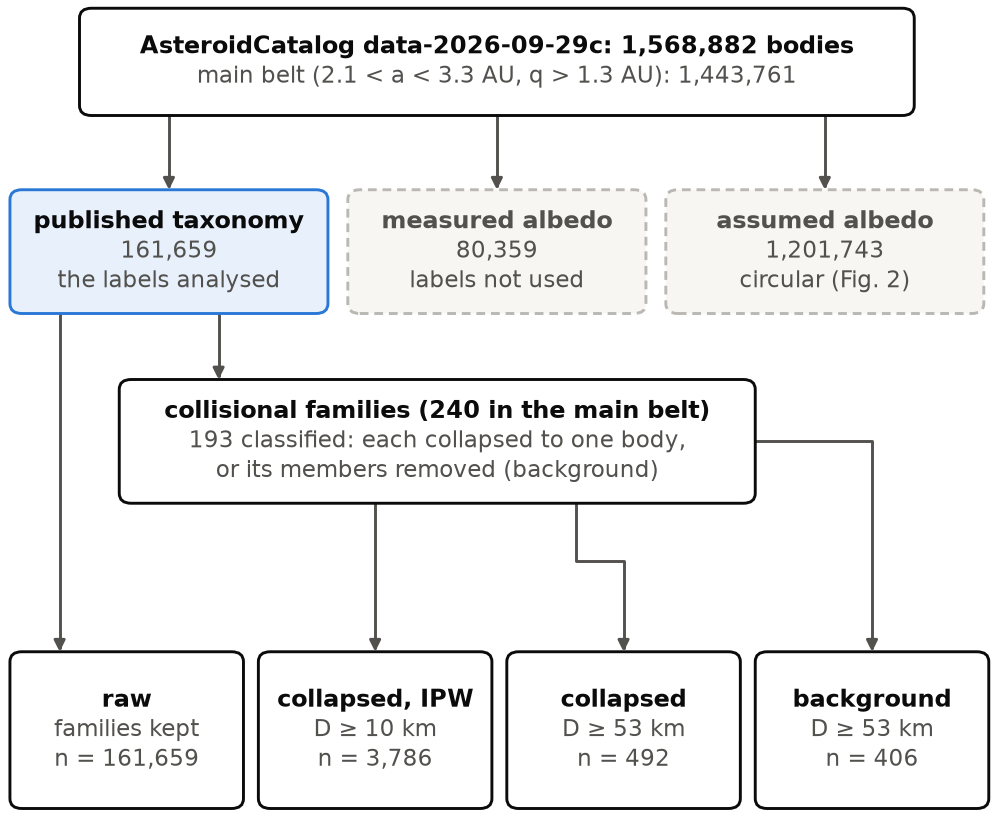
\includegraphics[width=\columnwidth]{figures/fig11_sample_flow.png}
\caption{Construction of the four samples from the catalog release, with the number of bodies at each step. Only the published taxonomy (highlighted) is analyzed; the two albedo-based routes are not used (Section~\ref{sec:3.1}).}\label{fig:3}
\end{figure}
\subsection{Fitting the S/C transition}\label{sec:3.5}
To locate the transition, a logistic model

\begin{equation}\label{eq:4}
P(\mathrm{C} \mid a) = \left[1 + e^{-(\beta_{0} + \beta_{1}(a - 2.7\,\mathrm{au}))}\right]^{-1}
\end{equation}
is fitted by weighted maximum likelihood to the S-like and C-like bodies of each sample. The crossover is $a_{50} = 2.7\ \mathrm{au} - \beta_{0}/\beta_{1}$, and the distance over which the C-fraction rises from 10\% to 90\% is $2 \ln 9/\beta_{1}$. Confidence intervals are derived from 200 bootstrap resamples.

\begin{figure*}[t!]
\centering
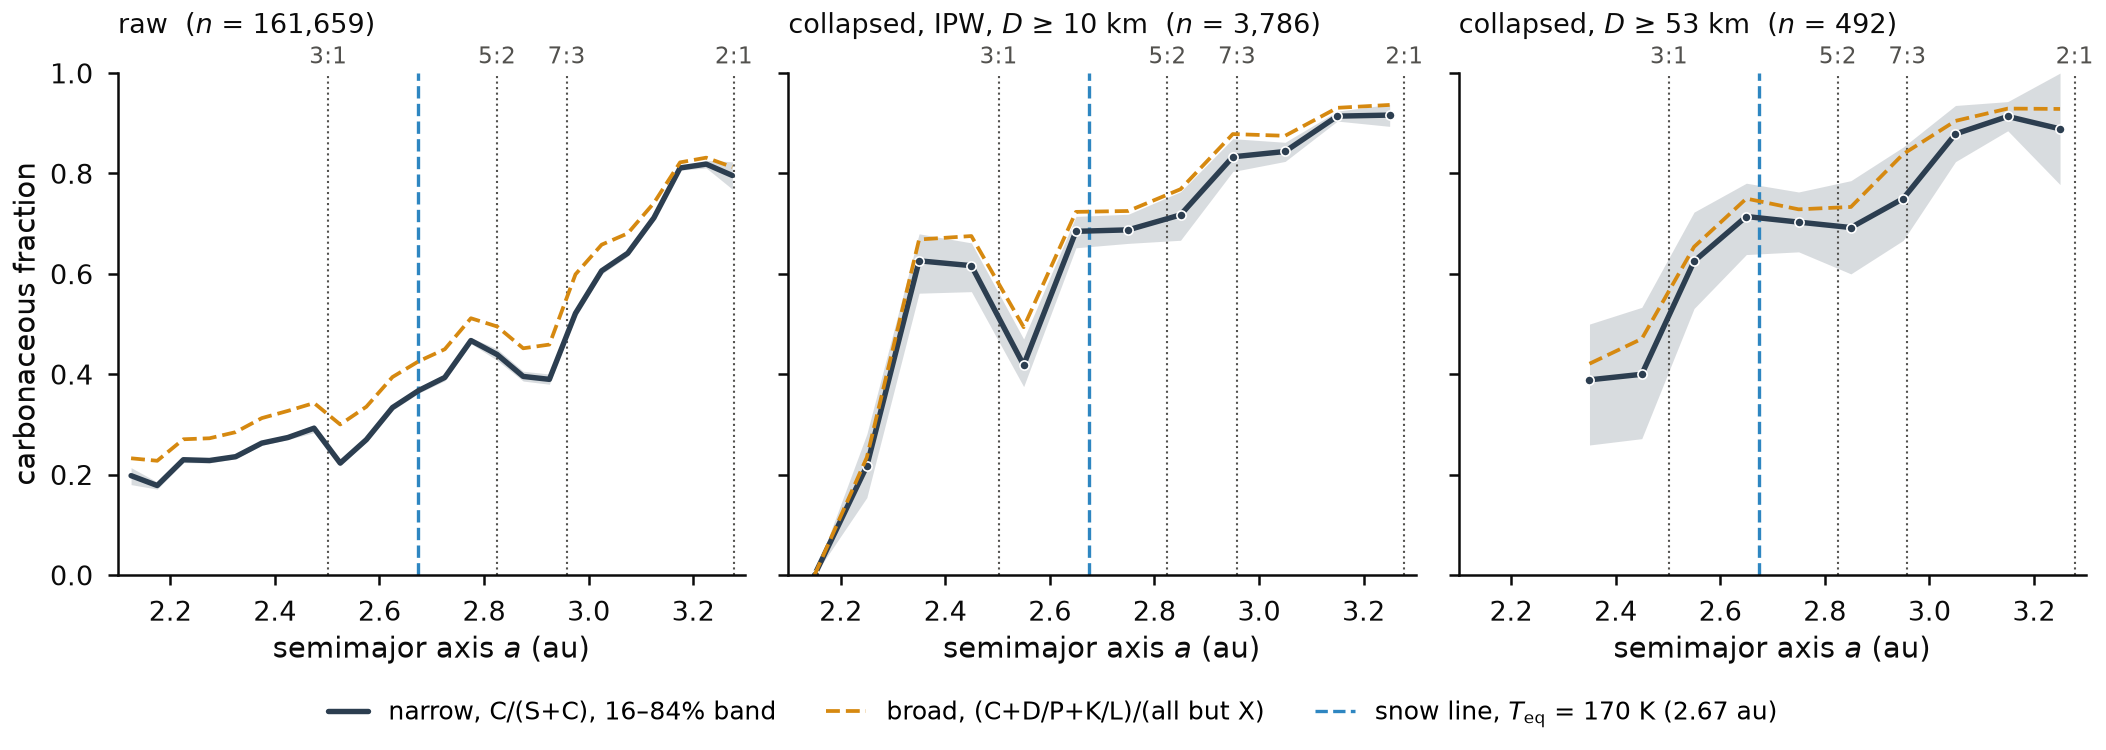
\includegraphics[width=\textwidth]{figures/fig1_c_fraction_vs_a.png}
\caption{Carbonaceous fraction versus semimajor axis. Left: every body with a published taxonomy. Center: families collapsed, weighted for completeness, $D \geq 10$~km. Right: families collapsed, complete sample, $D \geq 53$~km. Solid lines show the narrow fraction C/(S+C) with bootstrap 16–84\% bands; dashed lines show the broad fraction. Dotted lines mark the Kirkwood gaps; the blue dashed line marks the snow line of Equation~(\ref{eq:1}).}\label{fig:4}
\end{figure*}
\begin{deluxetable*}{lcccc}
\tabletypesize{\footnotesize}
\tablewidth{0pt}
\tablecaption{Narrow carbonaceous fraction C/(S+C) by zone.\label{tab:2}}
\tablehead{\colhead{Sample} & \colhead{Inner} & \colhead{Middle} & \colhead{Pristine} & \colhead{Outer}}
\startdata
Raw & 0.25 [0.24, 0.25] (49,691) & 0.35 [0.34, 0.35] (48,954) & 0.40 [0.39, 0.40] (5,155) & 0.70 [0.69, 0.70] (31,581) \\
Collapsed, IPW, $D \geq 10$~km & 0.53 [0.50, 0.56] (232) & 0.63 [0.61, 0.65] (658) & 0.77 [0.73, 0.80] (126) & 0.90 [0.89, 0.90] (1,248) \\
Collapsed, $D \geq 53$~km & 0.39 [0.32, 0.47] (38) & 0.69 [0.65, 0.73] (129) & 0.70 [0.62, 0.79] (30) & 0.89 [0.87, 0.92] (133) \\
Background, $D \geq 53$~km & 0.46 [0.35, 0.56] (24) & 0.71 [0.66, 0.75] (96) & 0.71 [0.61, 0.81] (21) & 0.91 [0.88, 0.93] (106)
\enddata
\tablecomments{Values are the fractions measured on the full sample, with 16–84\% bootstrap intervals in brackets; the number in parentheses is the number of S-like plus C-like bodies.}
\end{deluxetable*}
\subsection{Orbital excitation}\label{sec:3.6}
If inner-belt C-types were implanted from beyond Jupiter while inner-belt S-types formed nearby, the two populations could carry different dynamical histories in their eccentricities and inclinations. A belt that formed in place predicts no such difference. For each zone, the proper $e_{\mathrm{P}}$ and $\sin i_{\mathrm{P}}$ distributions of \mbox{S-like} and C-like background bodies (family members excluded) with $D \geq 10$~km are compared using a two-sample Kolmogorov–Smirnov (KS) test. With eight tests, the Bonferroni-corrected significance threshold is $p < 0.00625$.

\section{Results}\label{sec:4}
\subsection{The gradient is real but not sharp}\label{sec:4.1}
Figure~\ref{fig:4} and Table~\ref{tab:2} show the carbonaceous fraction as a function of semimajor axis. All samples show a gradient: C-types become more common with distance. However, the raw sample substantially understates how carbonaceous the belt is. It gives a narrow C-fraction of 0.25 in the inner belt and 0.35 in the middle belt. Once families are collapsed and the sample is limited by size, those values rise to 0.39–0.53 in the inner belt and 0.63–0.71 in the middle belt. The two debiasing methods, which use different size limits and different corrections, agree within their uncertainties in every zone except the inner belt, where the complete sample is small (38 bodies).

Two features of the debiased curves merit attention. The innermost belt, from 2.1 to about 2.3~au, remains mostly S-type after correction: the weighted C-fraction is 0 at 2.1–2.2~au and 0.22 at 2.2–2.3~au, and the complete samples contain only four or five bodies there. There is also a dip in the C-fraction just outside the 3:1 resonance at 2.55~au, visible in both the raw and IPW samples. This is the region of the large S-type Eunomia and Maria families, and the dip probably comes from family “halo” members that the HCM lists do not capture (\citealt{brozmorbidelli2013}; Section~\ref{sec:5.5}).

The broad fraction behaves the same way and is higher by 0.02–0.10 in every zone. Figure~\ref{fig:5} shows all five groups for the complete sample. D/P types are concentrated beyond the 7:3 resonance, where they make up 14–25\% of large bodies in each 0.1~au bin. X-types are common throughout, which underlines that their exclusion from the S/C ratio is a methodological choice.

\begin{figure}[htb!]
\centering
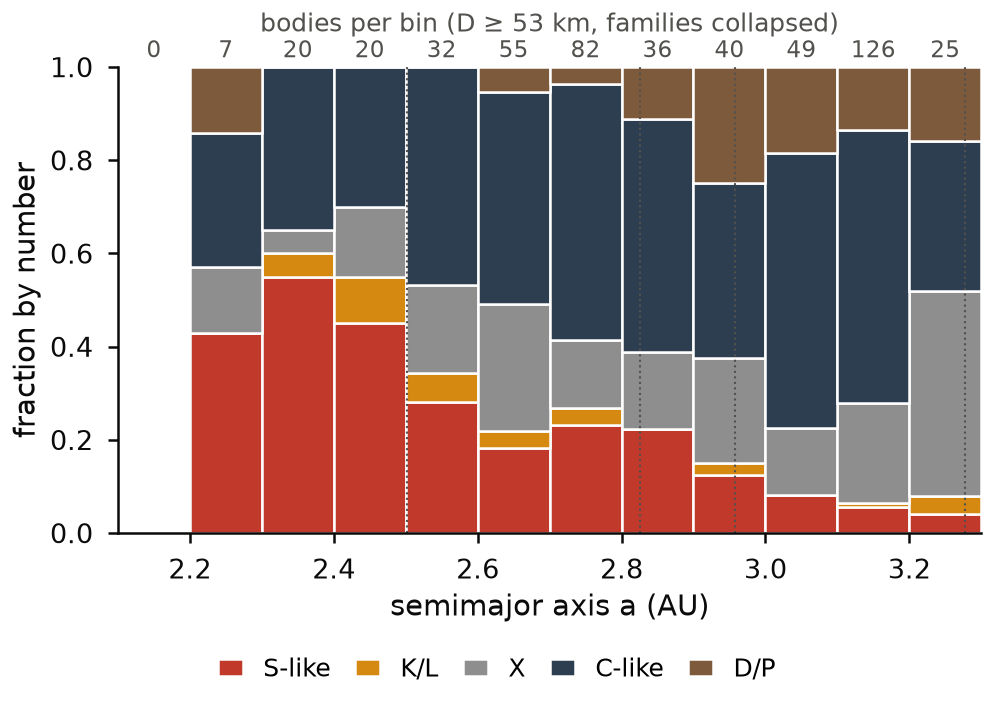
\includegraphics[width=\columnwidth]{figures/fig1b_stacked_composition.png}
\caption{Composition of the size-complete, family-collapsed sample ($D \geq 53$~km) in 0.1~au bins. The numbers above the plot give the number of bodies in each bin; dotted lines mark the Kirkwood gaps.}\label{fig:5}
\end{figure}
\subsection{Size dependence in the inner belt}\label{sec:4.2}
The inner-belt result depends on size in a way that matters for comparison with earlier work. Table~\ref{tab:3} splits the classified inner-belt bodies by diameter, with families included so that the numbers can be compared directly with \citet{demeo2014}. Above 100~km the inner belt is mostly S-type: 9 of 15 bodies are \mbox{S-like}, and C-types hold only 5\% of the mass. This is the classical picture of \citet{gradie1982}. Between 20 and 100~km, however, C-types are about as common as S-types (47\% at 50–100~km) or more so (60\% at 20–50~km). The “large-body” C-fractions in Table~\ref{tab:2} come from this 50–100~km range, not from the few largest bodies. Figure~\ref{fig:6} extends the comparison to the whole belt with the completeness-weighted sample. Between 2.3 and 2.5~au the inner belt is mixed at every size from 10 to 100~km, and S-types are in the majority only inside 2.3~au, at 2.5–2.6~au below 50~km, and at 2.3–2.4~au above 50~km.

\begin{deluxetable}{lcccc}
\tabletypesize{\footnotesize}
\tablewidth{0pt}
\tablecaption{Inner-belt (2.1–2.5~au) S-like and C-like bodies by diameter.\label{tab:3}}
\tablehead{\colhead{} & \colhead{} & \colhead{} & \multicolumn{2}{c}{C-fraction} \\ \cline{4-5}
\colhead{Diameter} & \colhead{$n_{\mathrm{S}}$} & \colhead{$n_{\mathrm{C}}$} & \colhead{by number} & \colhead{by mass}}
\startdata
$\geq 100$~km & 9 & 6 & 0.40 & 0.05 \\
50–100~km & 16 & 14 & 0.47 & 0.29 \\
20–50~km & 26 & 39 & 0.60 & 0.39 \\
5–20~km & 1,112 & 1,039 & 0.48 & 0.34
\enddata
\tablecomments{Families are included, as in \citet{demeo2014}. The 5–20~km bin is not debiased; the taxonomic sample favors bright S-types at these sizes, so its C-fraction is a lower limit.}
\end{deluxetable}
\begin{figure}[htb!]
\centering
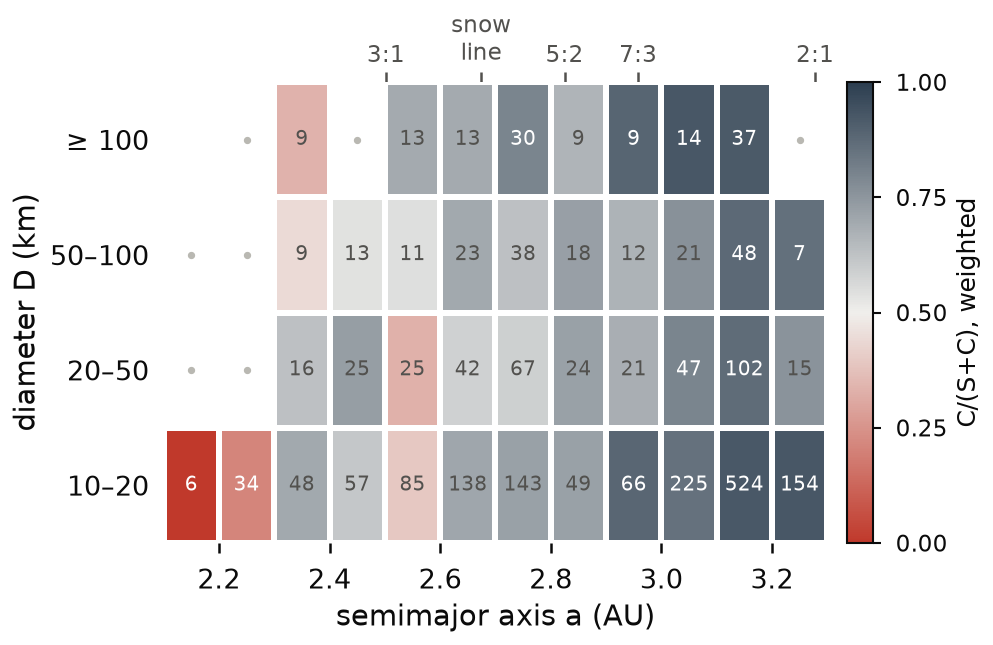
\includegraphics[width=\columnwidth]{figures/fig6_size_distance_map.png}
\caption{Narrow carbonaceous fraction C/(S+C) of the family-collapsed, completeness-weighted sample ($D \geq 10$~km) in cells 0.1~au wide in semimajor axis, for four ranges of diameter. Numbers give the \mbox{S-}~and C-type bodies in each cell; cells with fewer than five are left blank, and a dot marks those that hold any. Ticks on the top axis mark the Kirkwood gaps and the snow line of Equation~(\ref{eq:1}).}\label{fig:6}
\end{figure}
\subsection{By mass}\label{sec:4.3}
Asteroid masses have been measured, from spacecraft, binary orbits or gravitational perturbations, for only a few hundred bodies (\citealt{carry2012}). In this sample 370 classified bodies have a measured mass, and they hold 95\% of the classified mass; for the rest the catalog multiplies the volume by a bulk density typical of the taxonomic class (\citealt{edwards2026b}). Mass is dominated by a few bodies. Ceres alone holds 39\% of the mass of classified main-belt asteroids, Vesta 11\%, Pallas 9\% and Hygiea 3\% (Figure~\ref{fig:7}). Counting only \mbox{S-}~and C-types, the inner belt’s mass is 94\% S-like, almost entirely because of Vesta, and the middle belt’s is 91\% C-like, because of Ceres and Pallas. Removing these four bodies gives C mass fractions of 0.26, 0.50, 0.71 and 0.92 from the inner to the outer zone. Once the few largest bodies are set aside, the mass distribution is therefore consistent with the counts, but it is too dominated by individual objects to constrain a gradient on its own.

\begin{figure*}[t!]
\centering
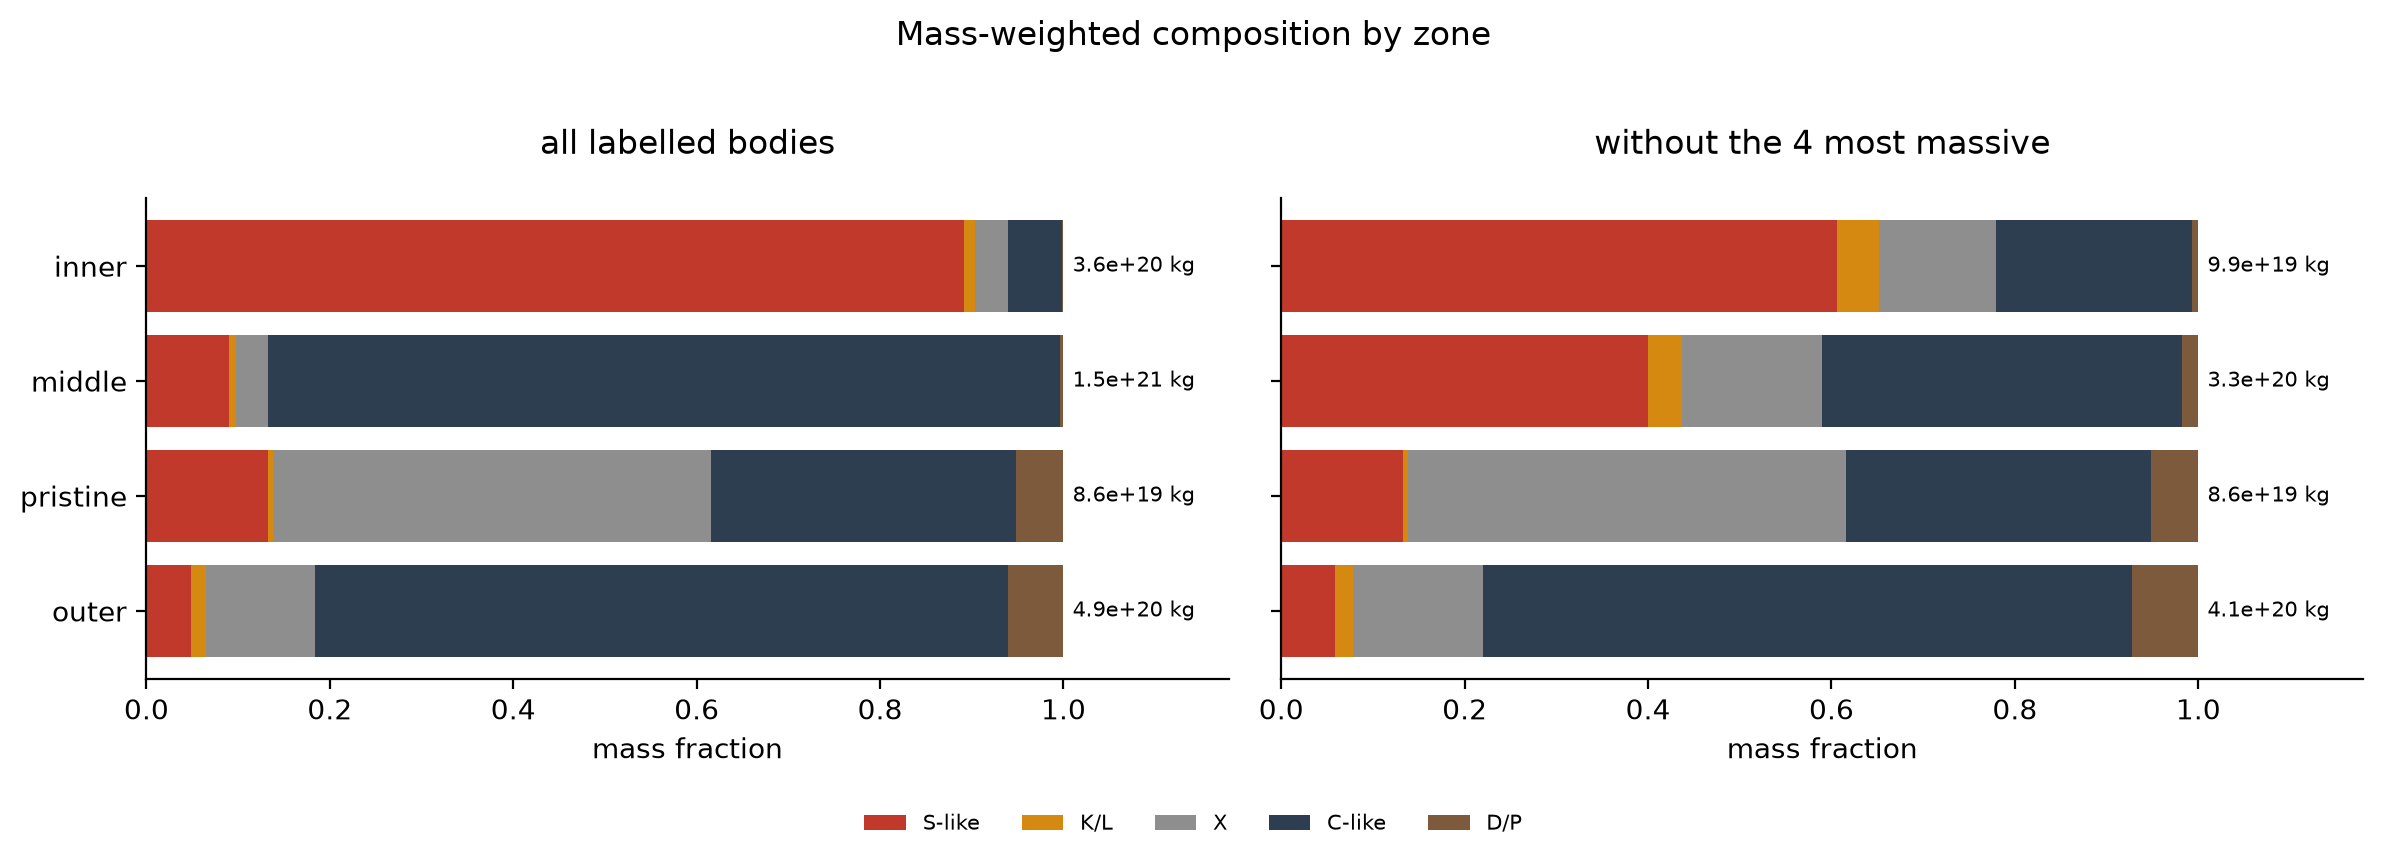
\includegraphics[width=\textwidth]{figures/fig2_mass_by_zone.png}
\caption{Mass fraction of each compositional group by zone, for all classified bodies (left) and without Ceres, Vesta, Pallas and Hygiea (right). Total classified mass per zone is given at right.}\label{fig:7}
\end{figure*}
\subsection{The crossover}\label{sec:4.4}
Table~\ref{tab:4} lists the fitted crossover for each sample, and Figure~\ref{fig:8} shows the fitted curves. The raw sample places it at 2.84~au, close to the classical snow line. The three debiased samples move it inward to 2.41–2.47~au, about 0.2~au inside the snow line of Equation~(\ref{eq:1}), and agree with each other within their uncertainties. In every debiased sample the 10–90\% width of the transition is 1.4–1.5~au, larger than the 1.2~au span of the belt. Because the width exceeds the belt, part of the fitted curve lies outside the range the data cover; in practice, the belt never becomes 90\% S-type at its inner edge and reaches 90\% C-type only in its outermost bins.

\begin{deluxetable*}{lccc}
\tabletypesize{\footnotesize}
\tablewidth{0pt}
\tablecaption{Logistic fit to the S/C transition.\label{tab:4}}
\tablehead{\colhead{Sample} & \colhead{$a_{50}$ (au)} & \colhead{10–90\% width (au)} & \colhead{$n_{\mathrm{S+C}}$}}
\startdata
Raw & 2.84 [2.84, 2.84] & 1.72 [1.70, 1.73] & 135,381 \\
Collapsed, IPW, $D \geq 10$~km & 2.46 [2.43, 2.49] & 1.39 [1.32, 1.48] & 2,264 \\
Collapsed, $D \geq 53$~km & 2.47 [2.39, 2.53] & 1.38 [1.18, 1.66] & 330 \\
Background, $D \geq 53$~km & 2.41 [2.31, 2.49] & 1.49 [1.21, 1.83] & 247 \\
Snow line, Equation~(\ref{eq:1}) & 2.67 & \nodata & \nodata
\enddata
\tablecomments{Intervals are 16–84\% bootstrap ranges. The width is the distance over which the fitted C-fraction rises from 10\% to 90\%. The snow-line row uses Equation~(\ref{eq:1}) with $T = 170$~K.}
\end{deluxetable*}
\begin{figure}[htb!]
\centering
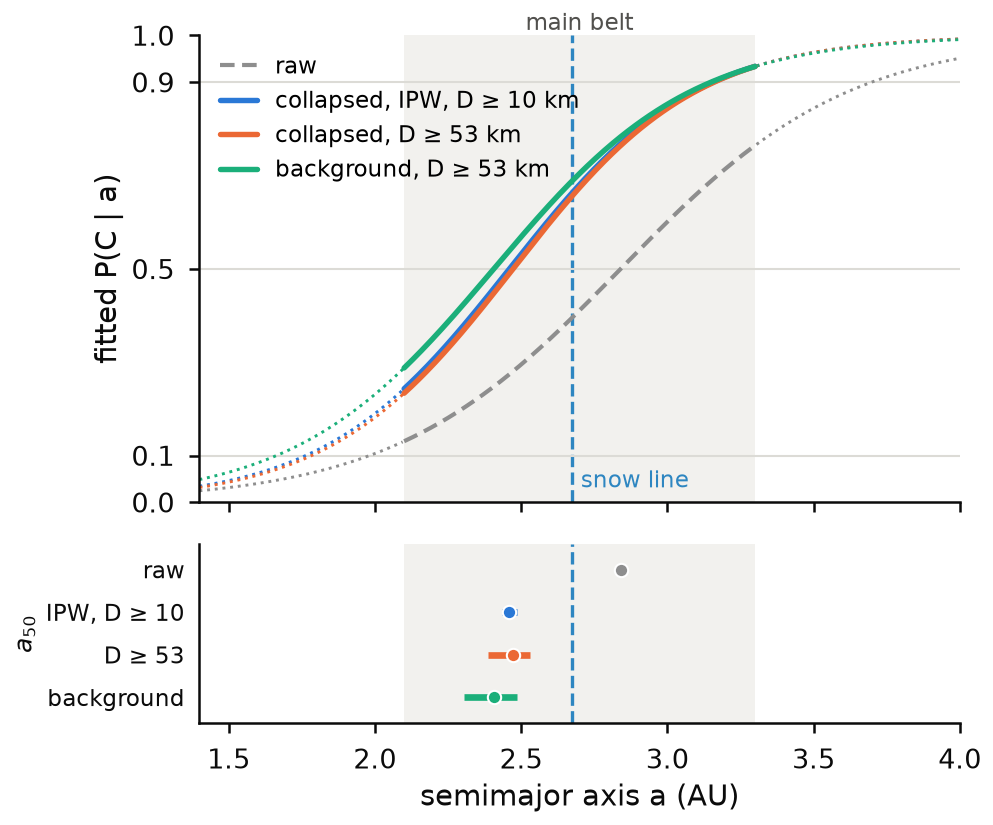
\includegraphics[width=\columnwidth]{figures/fig7_crossover_fits.png}
\caption{Logistic fits (Equation~(\ref{eq:4})) to the four samples of Table~\ref{tab:4}, solid within the main belt (shaded) and dotted outside it. The lower panel gives each crossover $a_{50}$ with its 16–84\% bootstrap interval; the dashed line marks the snow line of Equation~(\ref{eq:1}).}\label{fig:8}
\end{figure}
\subsection{Orbital excitation}\label{sec:4.5}
Figure~\ref{fig:9} and Table~\ref{tab:5} compare the proper orbits of \mbox{S-}~and C-types within each zone. In the inner belt, where the implantation question matters most, the two distributions are nearly identical ($p = 0.44$ for $e_{\mathrm{P}}$, 0.17 for $\sin i_{\mathrm{P}}$). The largest differences in median are in the pristine zone, where C-types have higher median eccentricity (0.175 versus 0.113) and inclination ($\sin i_{\mathrm{P}}$ 0.217 versus 0.125), but only 24 S-types fall in that zone and neither difference passes the corrected threshold. One test does pass it: the inclinations in the outer belt ($p = 0.0060$). Their medians are almost equal ($\Delta = 0.002$), and the distributions differ in shape: C-types show an excess at the lowest inclinations, where the C-type Themis family lies, and S-like bodies cluster near the inclination of the Eos family. Both patterns are expected from family members missing from the HCM lists (Section~\ref{sec:5.5}). Figure~\ref{fig:10} places the bodies of the test among the families: many outer-belt C-types lie at the low inclinations of the Themis family, and in the middle belt S-like background bodies concentrate around the Eunomia family. With the one-step family extension of Section~\ref{sec:4.6}, which attaches such bodies to their families, no test passes; the smallest $p$ is 0.011, again for the outer-belt inclinations.

\begin{figure*}[t!]
\centering
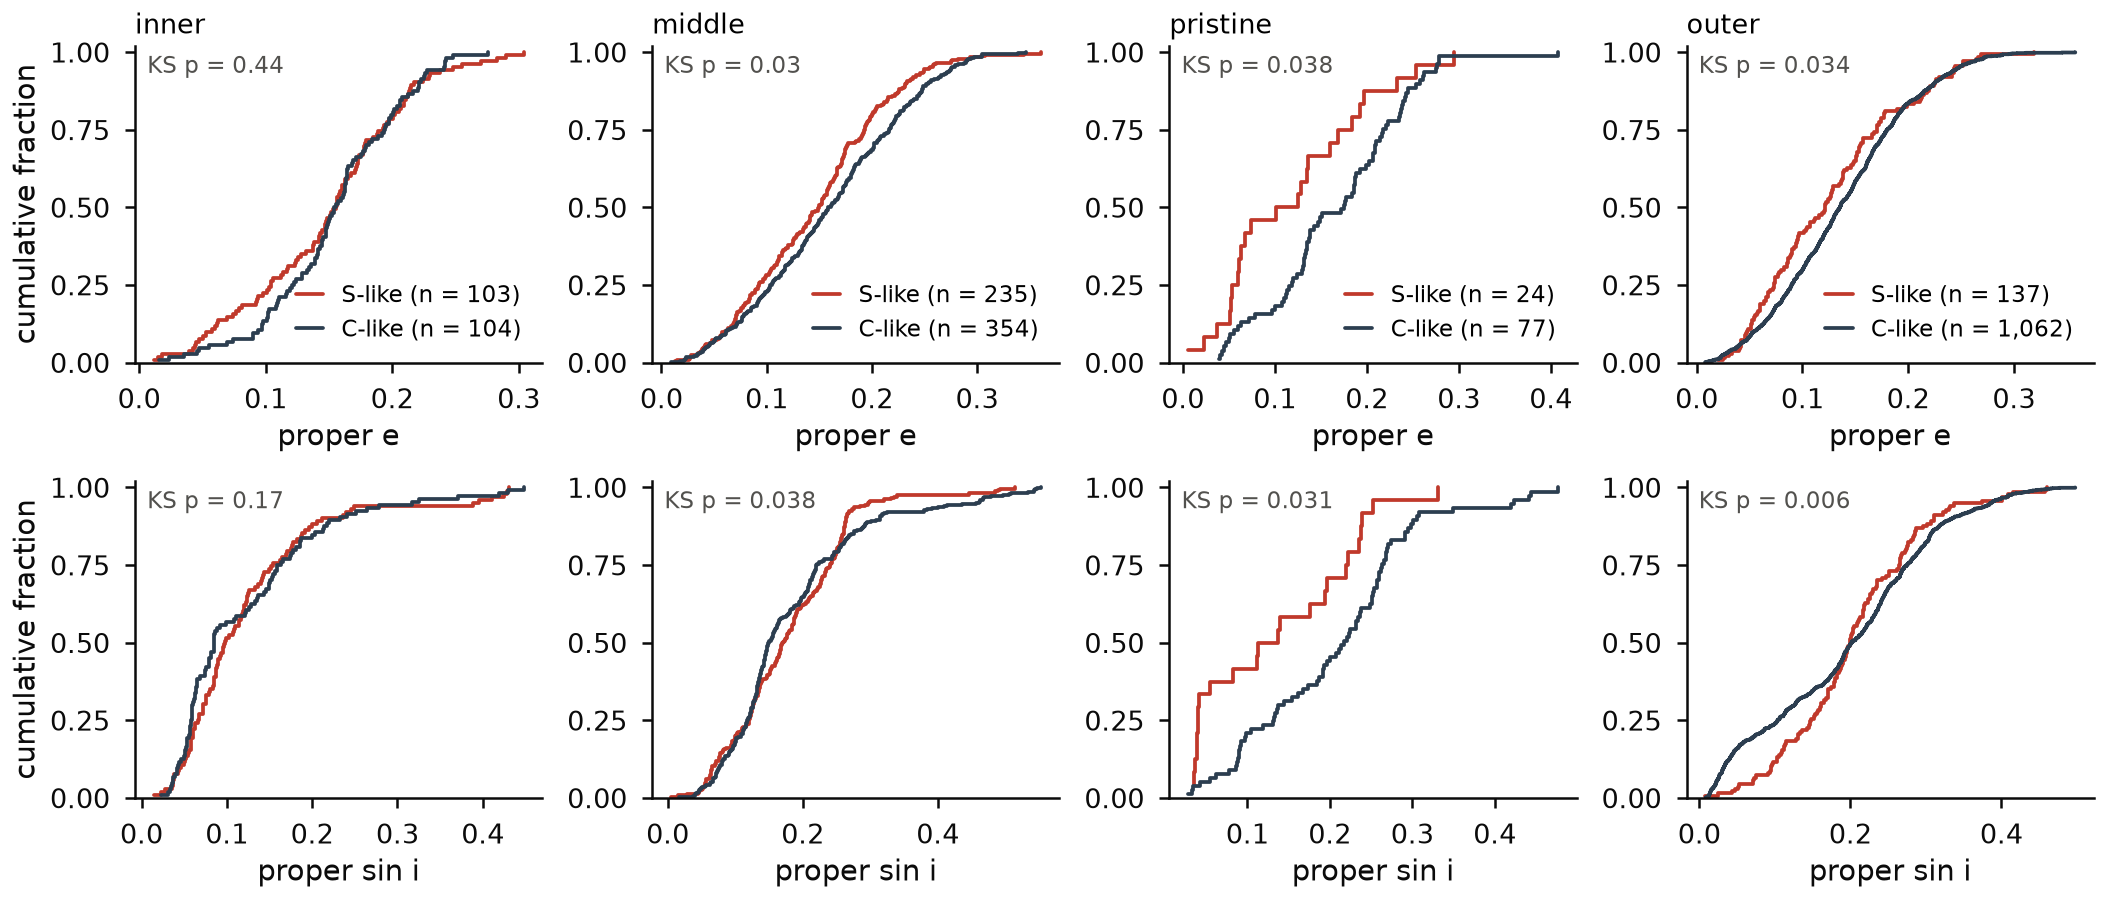
\includegraphics[width=\textwidth]{figures/fig3_orbital_excitation.png}
\caption{Cumulative distributions of proper eccentricity (top) and $\sin i$ (bottom) for S-like and C-like background bodies with $D \geq 10$~km, by zone. The Kolmogorov–Smirnov $p$-value is shown in each panel.}\label{fig:9}
\end{figure*}
\begin{deluxetable*}{lcccccc}
\tabletypesize{\footnotesize}
\tablewidth{0pt}
\tablecaption{Proper-element comparison of S-like and C-like background bodies with $D \geq 10$~km.\label{tab:5}}
\tablehead{\colhead{Zone} & \colhead{Element} & \colhead{$n_{\mathrm{S}}$} & \colhead{$n_{\mathrm{C}}$} & \colhead{$\Delta$} & \colhead{$D_{\mathrm{KS}}$} & \colhead{$p_{\mathrm{KS}}$}}
\startdata
Inner & $e_{\mathrm{P}}$ & 103 & 104 & \ensuremath{-}0.001 [\ensuremath{-}0.013, 0.017] & 0.12 & 0.44 \\
 & $\sin i_{\mathrm{P}}$ & 103 & 104 & \ensuremath{-}0.013 [\ensuremath{-}0.037, 0.023] & 0.15 & 0.17 \\
Middle & $e_{\mathrm{P}}$ & 235 & 354 & 0.010 [\ensuremath{-}0.004, 0.029] & 0.12 & 0.030 \\
 & $\sin i_{\mathrm{P}}$ & 235 & 354 & \ensuremath{-}0.021 [\ensuremath{-}0.038, \ensuremath{-}0.004] & 0.12 & 0.038 \\
Pristine & $e_{\mathrm{P}}$ & 24 & 77 & 0.062 [0.0002, 0.122] & 0.32 & 0.038 \\
 & $\sin i_{\mathrm{P}}$ & 24 & 77 & 0.092 [0.002, 0.172] & 0.33 & 0.031 \\
Outer & $e_{\mathrm{P}}$ & 137 & 1,062 & 0.014 [\ensuremath{-}0.002, 0.034] & 0.13 & 0.034 \\
 & $\sin i_{\mathrm{P}}$ & 137 & 1,062 & 0.002 [\ensuremath{-}0.014, 0.020] & 0.15 & 0.0060
\enddata
\tablecomments{$\Delta$ is median(C) \ensuremath{-} median(S) with a 95\% bootstrap interval. With eight tests, the Bonferroni-corrected threshold is $p < 0.00625$; only the outer-belt inclinations meet it.}
\end{deluxetable*}
\begin{figure}[htb!]
\centering
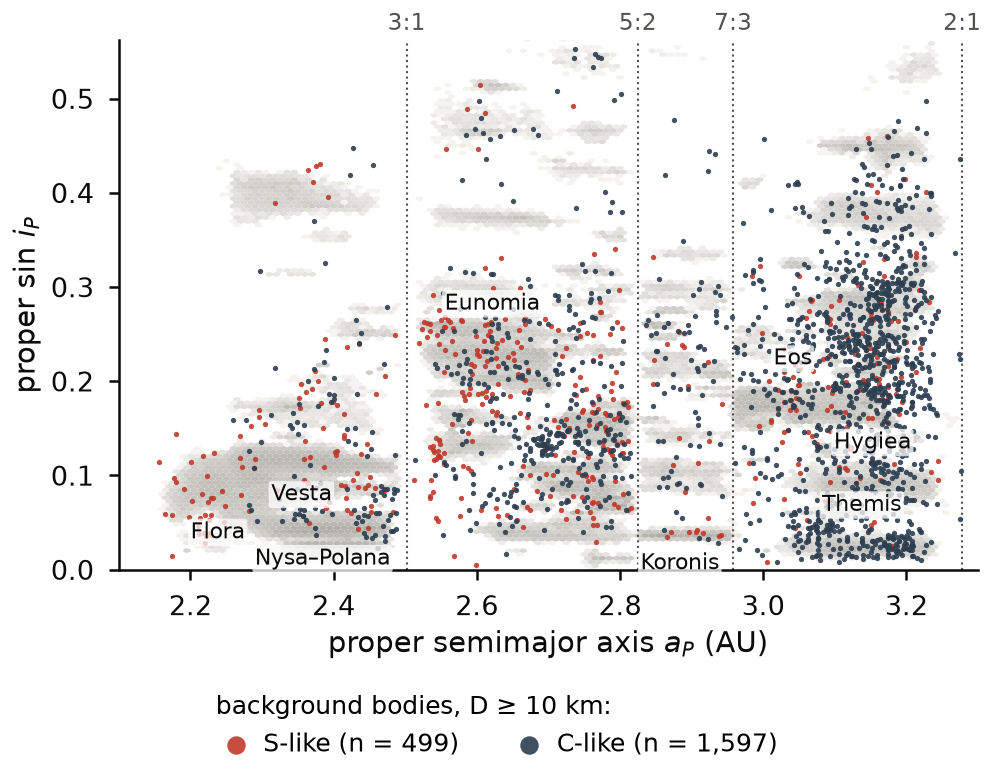
\includegraphics[width=\columnwidth]{figures/fig8_proper_elements.png}
\caption{Proper semimajor axis and inclination of the S-like and C-like background bodies with $D \geq 10$~km compared in Table~\ref{tab:5}, over the density of all family members (gray, logarithmic scale). Labels mark the largest families; dotted lines mark the Kirkwood gaps.}\label{fig:10}
\end{figure}
\subsection{Robustness}\label{sec:4.6}
\textbf{An albedo-only check. }Taxonomy can be avoided altogether by using measured albedos. C-, B-, \mbox{D-}~and T-types all have low visible albedos, while S-types are brighter, although the two overlap at small sizes (\citealt{mainzer2011b}). Treating $p_{\mathrm{V}} < 0.10$ as “dark” and applying the same completeness analysis gives a complete sample for $D \geq 33$~km. For background bodies in that sample, the dark fraction is 0.45, 0.66, 0.79 and 0.82 from the inner to the outer zone (Figure~\ref{fig:11}), in close agreement with the taxonomic results. Albedo and taxonomy come from different surveys and different physics (thermal infrared versus reflectance colors), so the agreement indicates that the result is not an artifact of the classification. The two measures are not identical: among bodies with both a published class and a measured albedo, 84\% of the C-like and 13\% of the S-like bodies are darker than 0.10 (Figure~\ref{fig:12}).

\begin{figure}[htb!]
\centering
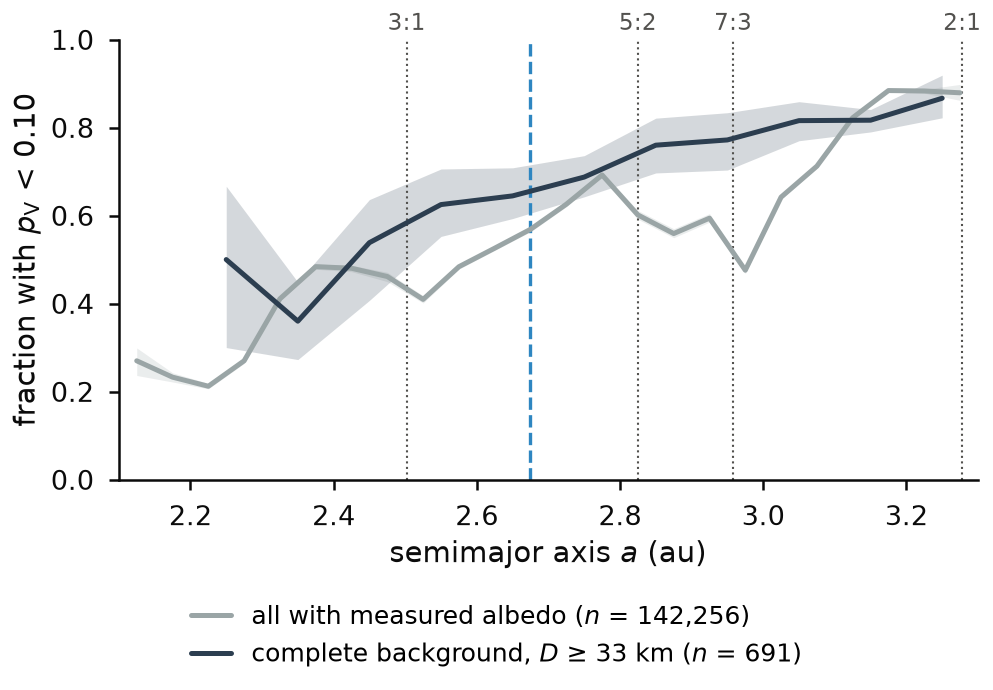
\includegraphics[width=\columnwidth]{figures/fig4_dark_fraction_albedo.png}
\caption{Fraction of bodies with measured geometric albedo $p_{\mathrm{V}} < 0.10$, for all bodies with a measured albedo (gray) and for the complete background sample, $D \geq 33$~km (dark). Shaded bands are 16–84\% bootstrap intervals; dotted lines mark the Kirkwood gaps and the dashed line the snow line of Equation~(\ref{eq:1}).}\label{fig:11}
\end{figure}
\textbf{Group definitions. }Switching from the narrow to the broad carbonaceous fraction raises every value by 0.02–0.10 and changes no conclusion.

\textbf{X-types by albedo. }By convention, an X-type with a measured albedo is a P-type below $p_{\mathrm{V}} = 0.10$, an M-type up to 0.30 and an E-type above (\citealt{fornasier2011}). Of the 13,763 classified X-complex bodies, 7,755 have a measured albedo and a label that does not already name the class (that is, not E, M, Xe or Xk), and 4,513 of these are P-like. Counting them with D/P, including in the family votes, raises the broad fraction by at most 0.06 and changes the narrow fraction by at most 0.01. The P-like share of these bodies is lower in the inner belt (0.38) than beyond it (0.54–0.66), in the same sense as the gradient in the other groups.

\begin{figure}[htb!]
\centering
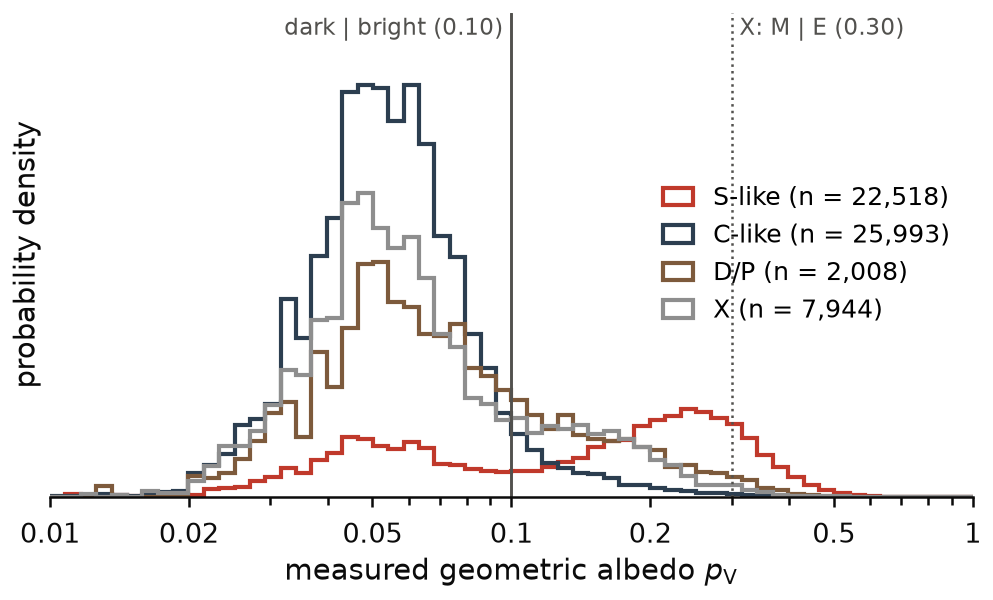
\includegraphics[width=\columnwidth]{figures/fig12_albedo_by_group.png}
\caption{Measured geometric albedo of the S-like, C-like, D/P and X-type bodies with a published taxonomy (normalized histograms). The solid line marks the dark/bright boundary of Section~\ref{sec:4.6} ($p_{\mathrm{V}} = 0.10$), and the dotted line the boundary between \mbox{M-}~and E-type X-types ($p_{\mathrm{V}} = 0.30$).}\label{fig:12}
\end{figure}
\textbf{Family membership. }The 2015 family lists include only asteroids numbered by 2015. As an upper bound on missed members, every unlisted body whose nearest listed family member lies within that family’s HCM cutoff is attached to that family. This is deliberately aggressive, since the cutoffs were tuned on a catalog of 384,337 numbered asteroids (\citealt{nesvorny2015}), about a third the size of the 1.25 million orbits used here, and it raises the family fraction from 10.6\% to 24.3\%. Even so, zone fractions change by at most 0.01 and the crossover moves by at most 0.02~au. Figure~\ref{fig:13} collects every per-zone estimate of Table~\ref{tab:2} and of this section: each rises from the inner to the outer belt, and only the raw count and the brightness-limited sample lie well below the others in the inner and middle belt.

\begin{figure}[htb!]
\centering
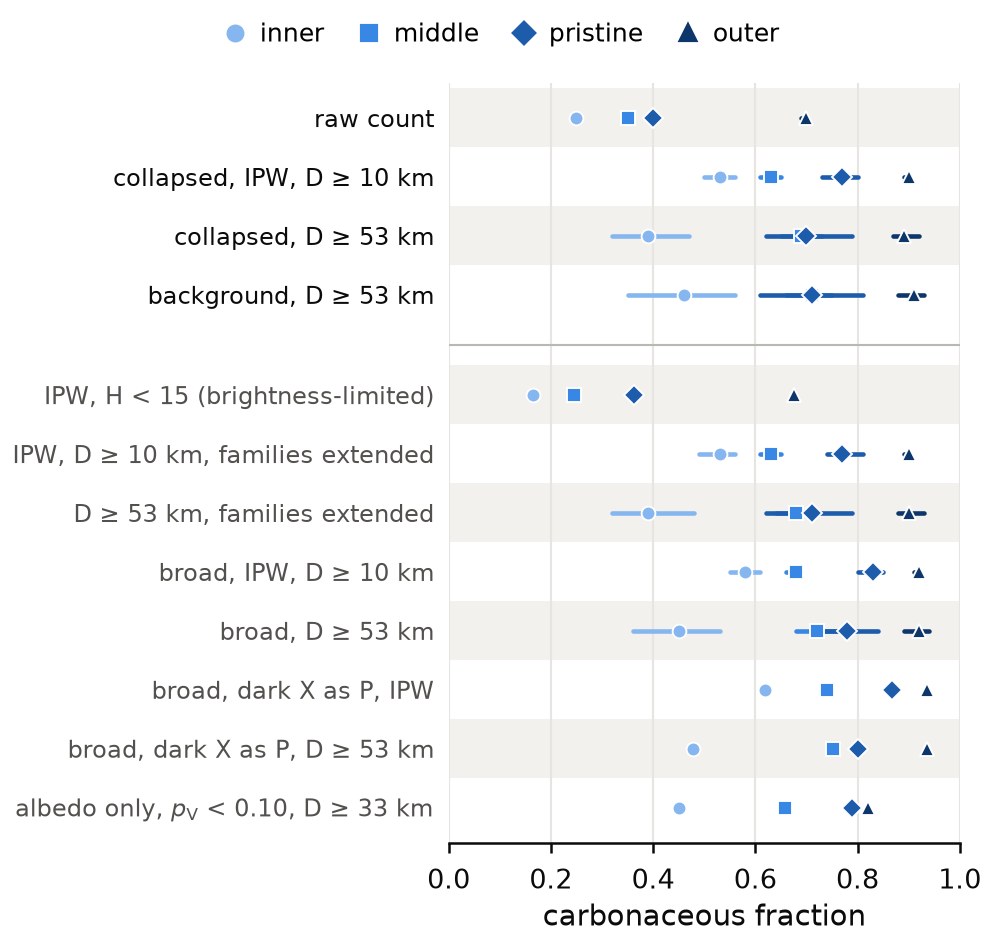
\includegraphics[width=\columnwidth]{figures/fig9_robustness.png}
\caption{Every per-zone carbonaceous fraction reported in this paper. The upper four rows are the samples of Table~\ref{tab:2}, with 16–84\% bootstrap intervals. The lower rows are the checks: the brightness-limited sample of Section~\ref{sec:3.4}, the one-step family extension, the broad fraction, the broad fraction with dark X-types counted as P-types, and the dark fraction from measured albedos (Section~\ref{sec:4.6}). Rows without intervals are point estimates.}\label{fig:13}
\end{figure}
\section{Discussion}\label{sec:5}
\subsection{A static front is ruled out; \texorpdfstring{\\*}{}a moving one is not enough}\label{sec:5.1}
A static condensation front predicted a transition much narrower than the belt, with an inner belt that is almost entirely S-type. Neither prediction is borne out. In every debiased sample the transition is wider than the belt, and between about 10 and 100~km roughly half of inner-belt bodies are carbonaceous (Figure~\ref{fig:6}). The albedo check shows this is not an artifact of the taxonomy.

A snow line that moved inward over the disk’s lifetime (Section~\ref{sec:2.2}) is harder to dismiss on these data alone. It would broaden the transition, and bodies that formed late in the inner belt could have accreted ice, provided icy particles still reached them from farther out (\citealt{morbidelli2016}). It cannot, however, change the origin of the material. The NC–CC split is recorded in nucleosynthetic isotope anomalies, which are inherited from the dust and are not reset by condensing or evaporating water (\citealt{kleine2020}). A hydrated body that formed at 2.3~au under a late, cold snow line would still consist of NC material. Every C-complex asteroid with a firm meteorite link, most directly Ryugu and Bennu (\citealt{yokoyama2023}; \citealt{lauretta2024}), samples carbonaceous-chondrite material instead. The carbonaceous bodies in the inner belt are therefore not locally formed ice-bearing rocks; they came from the CC reservoir, which lay beyond Jupiter while its core grew (\citealt{kruijer2017}), or beyond a pressure maximum near its orbit (\citealt{brasser2020}).

The crossover location deserves particular care, because it is the number most likely to be over-interpreted. The raw catalog places it at 2.84~au, close enough to the 2.7~au snow line to be mistaken for confirmation. That agreement is an artifact: once families and brightness bias are corrected, the crossover moves inward by about 0.4~au. Even the corrected value is not the location of a snow line. It marks where two delivered and then depleted populations happen to balance today.

\subsection{Comparison with DeMeo \& Carry (2014)}\label{sec:5.2}
\citet{demeo2014} mapped the belt by mass down to 5~km and concluded that every asteroid type is present in every region, with the mixing strongest at small sizes. They report that C-types make up only 6\% of inner-belt mass at large sizes, rising to about half at the smallest sizes. The present analysis agrees on the large-size number: the mass-weighted C-fraction of the inner belt is 6\% (Section~\ref{sec:4.3}), and 5\% for bodies above 100~km (Table~\ref{tab:3}). Both figures are set largely by Vesta.

The two analyses differ in emphasis rather than substance. Weighting by mass hides the 50–100~km population, which is negligible relative to Vesta but is already about half carbonaceous by number. DeMeo \& Carry emphasize the contrast between an orderly belt at the largest sizes and a mixed one at the smallest, where their inner-belt C mass fraction reaches one-half. The counts here (Table~\ref{tab:3}; Figure~\ref{fig:6}) show that the mixed population extends to sizes just below those of the few largest bodies. This distinction matters for interpretation. Bodies of 50–100~km are too large to have drifted far by the Yarkovsky effect over the age of the Solar System (\citealt{bottke2006}; \citealt{demeo2014}), so their mixing is more plausibly primordial than the mixing of small bodies. \citet{delbo2017} reach a consistent conclusion: the original planetesimals they identify among the inner belt’s dark asteroids, the bodies that belong to no family, are all larger than 35~km.

\subsection{Implantation fits the data}\label{sec:5.3}
Both implantation models reproduce the observations: broad overlap of the two populations, S-types more common inward and C-types outward, and carbonaceous material in the inner belt (\citealt{walsh2012}; \citealt{raymond2017b}). The concentration of D/P types beyond the 7:3 resonance (Figure~\ref{fig:5}) is also what the capture of trans-Neptunian objects predicts (\citealt{levison2009}; \citealt{vokrouhlicky2016}), although the present sample does not reach the Hildas and Trojans, where that prediction is strongest (\citealt{morbidelli2005}; \citealt{vokrouhlicky2016}). The meteorite record is interpreted in the same way: the growth of Jupiter scattered CC bodies inward, which is why NC and CC bodies now share the belt (\citealt{kleine2020}). The data do not distinguish the Grand Tack from the empty-belt model, nor from models that deplete and excite the belt without a migrating Jupiter (\citealt{izidoro2016}; \citealt{clement2019}), as long as the carbonaceous material arrives from beyond Jupiter. The Grand Tack and the empty-belt model both fill the belt from both directions, and what distinguishes them (whether Jupiter migrated, and how much mass the belt started with) is not recorded in the present-day composition gradient.

\subsection{Why the orbits do not distinguish the scenarios}\label{sec:5.4}
The near-null result of the orbital test is informative but not decisive. Whatever process excited the belt’s eccentricities and inclinations acted on both populations after they were in place (\citealt{petit2001}; \citealt{morbidelli2015}), and over 4.5~Gyr, secular resonances, mean-motion resonances and size-dependent Yarkovsky drift (\citealt{bottke2006}) would erase much of any small difference that survived. In the Grand Tack, for example, the eccentricities left by implantation are reshaped by the later giant-planet instability and 4~Gyr of evolution into a distribution close to today’s (\citealt{deienno2016}). The absence of a class dependence beyond what family halos produce is therefore consistent with implantation but does not independently favor it. The nominal excess excitation of pristine-zone C-types (Table~\ref{tab:5}) warrants re-examination with a larger S-type sample.

\subsection{Limitations}\label{sec:5.5}
\begin{itemize}
\item \textbf{Photometric taxonomy is coarse.} Most classifications come from SkyMapper or SDSS colors rather than spectra (\citealt{sergeyev2021}; \citealt{sergeyev2022}), so the analysis is kept at the level of broad groups. K-types are often confused with S-types in color data, which is why \citet{demeo2013} reclassify the K-type Eos family by hand; here Eos is classified as S-like by its majority (purity 0.44).
\item \textbf{The isotopic argument rests on a few sample links.} Section~\ref{sec:5.1} assumes that C-complex asteroids in general sample CC material. That is established for Ryugu and Bennu (\citealt{yokoyama2023}; \citealt{lauretta2024}) and supported by spectral links to CI and CM chondrites (e.g., \citealt{rivkin2012}), but not demonstrated body by body.
\item \textbf{Family lists are incomplete.} Halo members that the HCM cutoffs miss leak into the “background” (\citealt{brozmorbidelli2013}). Attaching new members to family cores, as \citet{milani2014} do, recovers more of them; the one-step extension in Section~\ref{sec:4.6} is a simple version of that approach. The dip near 2.55~au is probably an example, and the outer-belt inclination difference of Section~\ref{sec:4.5} (Figure~\ref{fig:10}) another. Very old families are more difficult still to identify, because their members have spread too far to cluster in proper elements. \citet{delbo2017} found a 4-billion-year-old family across the inner belt that contains most of its dark asteroids previously unlinked to families, and \citet{dermott2018} estimate that about 85\% of inner-belt asteroids come from the Flora, Vesta, Nysa, Polana and Eulalia families. Fragments of the dark ancient family would count here as independent background bodies. They would raise the inner-belt C-fraction of the $D \geq 10$~km sample more than that of the $D \geq 53$~km sample, which may be part of why the two differ most in the inner belt (0.53 and 0.39). Some families are also composites: Nysa–Polana contains an S-type and a C-type family (\citealt{walsh2013}), and Flora’s largest listed member is (9) Metis, an \mbox{M-type} body larger than the S-type (8) Flora itself, and almost certainly an interloper (classes and sizes from \citealt{edwards2026b}).
\item \textbf{Many diameters are derived.} Of the classified bodies, 62\% have diameters that the catalog derives from Equation~(\ref{eq:3}) with an albedo typical of their class (\citealt{edwards2026b}), not a measured size. Errors in those diameters blur the size cuts. The absolute magnitudes carry systematic errors of their own: catalog values for small asteroids were found to be too bright by 0.4–0.5~mag near $H \approx 14$ (\citealt{pravec2012}), which would shift both the derived diameters and the $H$ bins of the completeness correction.
\item \textbf{The weighting assumes classification is class-blind.} The IPW method assumes that at fixed $H$ and zone, whether a body has been classified does not depend on its type. The size-complete sample does not require this assumption and yields the same result.
\end{itemize}
\section{Conclusions}\label{sec:6}
\begin{enumerate}
\item After collapsing collisional families and limiting the sample by size, the narrow carbonaceous fraction C/(S+C) is 0.39–0.53 in the inner belt and 0.63–0.71 in the middle belt, depending on the sample, well above the raw values of 0.25 and 0.35. The few inner-belt bodies above 100~km remain mostly S-type.
\item The S/C crossover lies at $a_{50} = 2.41$–2.47~au, and the transition is 1.4–1.5~au wide, wider than the belt. The raw catalog’s crossover at 2.84~au, close to the classical snow line, is an artifact of families and brightness bias.
\item A taxonomy-free check using measured albedos reproduces the gradient, counting dark X-types as P-types changes no conclusion, and the large-body mass fractions agree with \citet{demeo2014}.
\item \mbox{S-}~and C-types show no significant difference in proper eccentricity or inclination in any zone, except an outer-belt inclination difference that disappears once likely family-halo members are removed.
\item A static condensation front is ruled out by the width of the transition. A snow line that moved inward could broaden it, but cannot place isotopically carbonaceous material in the inner belt. The data therefore favor implantation of carbonaceous bodies from beyond Jupiter, but cannot distinguish the Grand Tack from the empty-belt model, or either from models that deplete the belt without a migrating Jupiter.
\end{enumerate}
A secondary conclusion is methodological. More than four-fifths of the main-belt labels in the catalog used here were inferred from an albedo assigned by distance, and would have reproduced the very gradient under test. Before a large catalog is used to test a hypothesis, it should be established how each value in it was obtained.

\begin{acknowledgments}
This research has made use of data and services provided by the International Astronomical Union’s Minor Planet Center; of the SsODNet service of IMCCE, Observatoire de Paris (\citealt{berthier2023}); and of the Minor Planet Physical Properties Catalogue (MP3C) of the Observatoire de la Côte d’Azur. This publication also makes use of data products from NEOWISE, which is a project of the Jet Propulsion Laboratory/California Institute of Technology, funded by the Planetary Science Division of the National Aeronautics and Space Administration.

\end{acknowledgments}
\software{NumPy \citep{harris2020}, SciPy \citep{virtanen2020}, pandas \citep{mckinney2010}, Matplotlib \citep{hunter2007}, asteroid-belt-gradient \citep{edwards2026a}}
\section*{Data availability}
{\raggedright % URLs and identifiers cannot stretch: ragged right instead of loose justified lines
Family membership and proper elements: the PDS Small Bodies Node, bundle \texttt{ast.nesvorny.families} V2.0 (\citealt{nesvorny2024}). Asteroid catalog: the AsteroidCatalog (\citealt{edwards2026b}; \url{https://github.com/loggger101/AsteroidCatalog}), release \mbox{data-2026-09-29c}, one frozen build that the analysis code downloads by its tag. Among its sources is the NEOWISE Diameters and Albedos V2.0 data set (\citealt{mainzer2019}). Analysis code: asteroid-belt-gradient v2.6.3 (\citealt{edwards2026a}; \url{https://github.com/loggger101/asteroid-belt-gradient}), which downloads both inputs and reproduces every figure and table; every number in the text that comes from the data or from the calculations described here is written to its \texttt{results/summary.json}.\par}

\appendix
\restartappendixnumbering
\section{Completeness of the taxonomic sample}\label{app:completeness}
\begin{figure}[htb!]
\centering
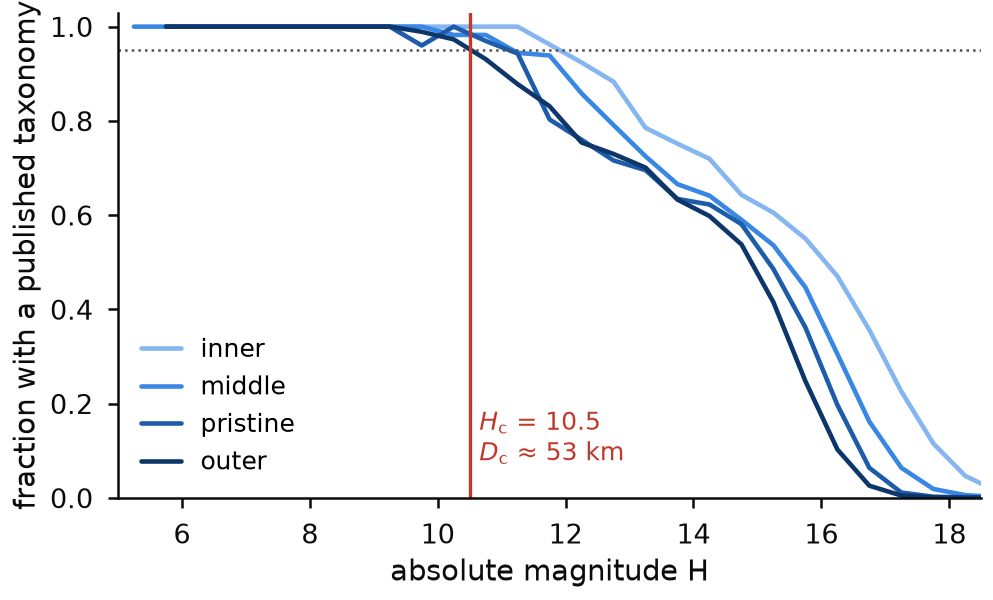
\includegraphics[width=3.3125in]{figures/fig0_completeness.png}
\caption{Fraction of main-belt bodies with a published taxonomy, by absolute magnitude and zone. The red line marks $H_{\mathrm{c}} = 10.5$, brighter than which every bin in every zone is at least 95\% classified; the dotted line marks 95\%.}\label{fig:A1}
\end{figure}
\bibliography{refs}{}
\bibliographystyle{aasjournalv7tie}
\end{document}
